\chapter{Manual de Mantenimiento del Sistema}
\label{AppendixC}
\label{AppendixC:Manual}

Este apéndice documenta los procedimientos operativos de mantenimiento del sistema de firma electrónica desplegado en la FACET. Su propósito es complementar la Sección~\ref{sec:validacion_respaldo} del Capítulo~\ref{chap:ensayos_resultados}, concentrando el detalle paso a paso de las tareas de restauración en un único documento de referencia para el personal de TI.

Los procedimientos descritos asumen que los artefactos de respaldo (volcados \texttt{.dmp} y archivos \texttt{.tar.gz}) se encuentran disponibles en los buckets correspondientes del servidor MinIO, tal como se verifica en la Sección~\ref{sec:validacion_respaldo}.

%----------------------------------------------------------------------------------------

\section{Restauración de la Base de Datos}
\label{AppendixC:RestauracionBD}

Este procedimiento permite restaurar PostgreSQL a partir de un volcado \texttt{.dmp} almacenado en el \textit{bucket} \texttt{documenso-backup-databases} de MinIO. La operación se ejecuta íntegramente desde la interfaz de Coolify y no requiere acceso directo por terminal al contenedor de la base de datos.

\textbf{Prerrequisitos:} acceso al panel de Coolify con permisos de administrador y conectividad con el servidor MinIO.

\begin{enumerate}
    \item \textbf{Localizar el respaldo.} Dentro de Coolify, navegar al proyecto Documenso siguiendo la ruta \texttt{Documenso} $\rightarrow$ \texttt{production} $\rightarrow$ \texttt{DocumensoProd}. Seleccionar el servicio de la base de datos (\texttt{database (postgres:17)}) y acceder a la pestaña \textbf{Backups}. En el listado de ejecuciones, identificar el último respaldo con estado \texttt{Success} y copiar la ruta completa indicada en el campo \texttt{Location} (Figura~\ref{fig:apC_backup_location}).

    \begin{figure}[H]
        \centering
        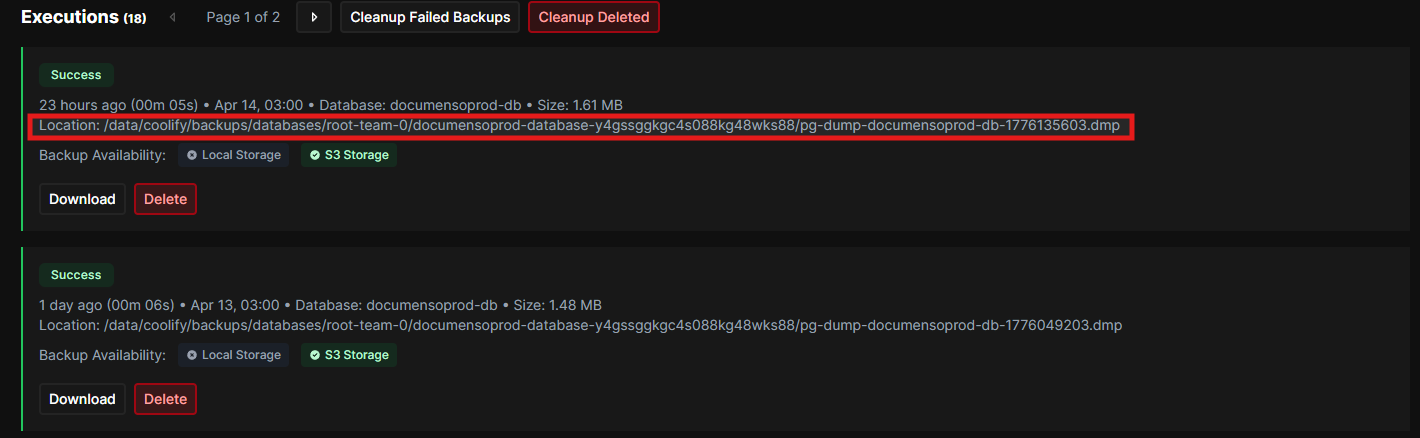
\includegraphics[width=\textwidth]{figuras/apendiceC/C1/apC-backup-location.png}
        \caption[Historial de respaldos de PostgreSQL en Coolify]{Pestaña \textbf{Backups} del servicio \texttt{database} en Coolify. Se observan las ejecuciones diarias con estado \texttt{Success}, el tamaño de cada volcado y el campo \texttt{Location} que contiene la ruta del objeto en MinIO.}
        \label{fig:apC_backup_location}
    \end{figure}

    \item \textbf{Configurar la importación.} Acceder a la pestaña \textbf{Import Backup} del mismo servicio. En la sección \textbf{Choose Restore Method}, seleccionar la opción \textbf{Restore from S3}.

    \item \textbf{Seleccionar el origen S3.} En el menú desplegable \texttt{S3 Storage}, elegir la conexión previamente configurada en Coolify: \textit{Backup Sistemas de Firmas -- Respaldo del Sistema de Firmas Documenso}.

    \item \textbf{Validar el archivo.} En el campo \texttt{S3 File Path (within bucket)}, pegar la ruta (\texttt{Location}) copiada en el paso~1. Presionar el botón \textbf{Check File} y verificar que la sección \textbf{File Information} muestre el nombre y el tamaño del volcado. Esta comprobación confirma que el objeto existe en MinIO y que la conexión S3 es funcional.

    \item \textbf{Modificar el comando de restauración.} Este es el paso más crítico del procedimiento. El comando de importación que Coolify genera por defecto es:

    \begin{quote}
    \texttt{pg\_restore -U \$POSTGRES\_USER -d \$\{POSTGRES\_DB:-\$\{POSTGRES\_USER:-postgres\}\}}
    \end{quote}

    \textbf{Advertencia:} si la base de datos de destino ya contiene datos ---que es el caso habitual en un entorno de producción activo---, la ejecución sin modificaciones fallará por colisión de objetos existentes. El administrador \textbf{debe} agregar la bandera \texttt{-{}-clean} al final del campo \texttt{Custom Import Command} para que \texttt{pg\_restore} elimine los objetos de la base antes de recrearlos. El comando final debe quedar de la siguiente forma:

    \begin{quote}
    \texttt{pg\_restore -U \$POSTGRES\_USER -d \$\{POSTGRES\_DB:-\$\{POSTGRES\_USER:-postgres\}\} -{}-clean}
    \end{quote}

    \item \textbf{Ejecutar la restauración.} Una vez configurados los campos anteriores, presionar el botón \textbf{Restore Database from S3} (Figura~\ref{fig:apC_import_backup}). Coolify descargará el volcado desde MinIO y ejecutará \texttt{pg\_restore -{}-clean} contra el contenedor de PostgreSQL.

    \begin{figure}[H]
        \centering
        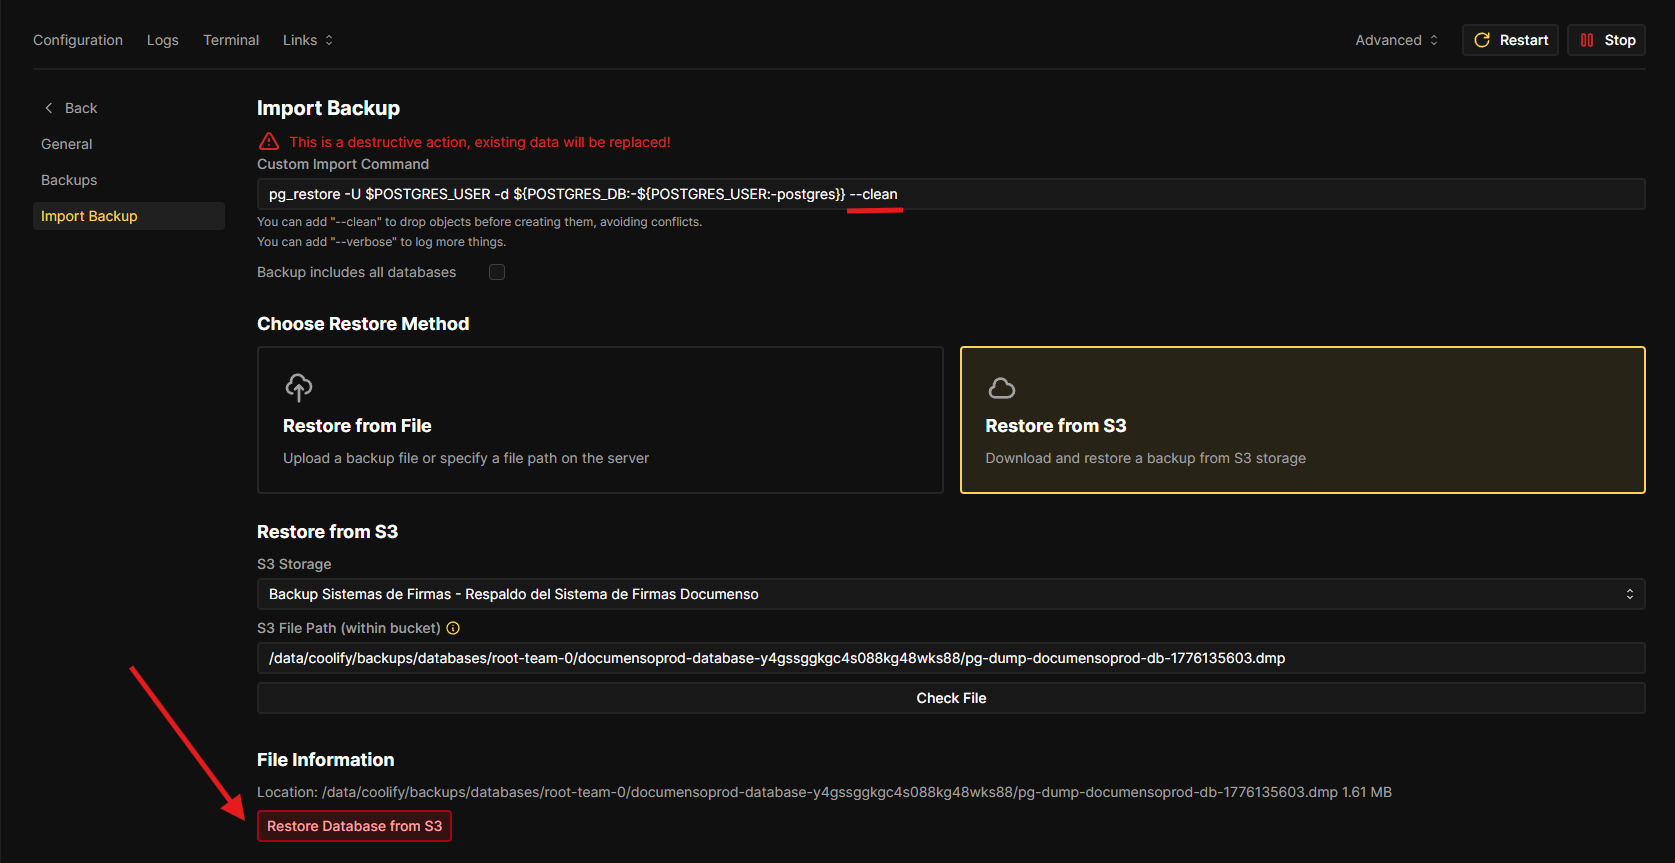
\includegraphics[width=\textwidth]{figuras/apendiceC/C1/apC-import-backup.png}
        \caption[Formulario de importación de respaldo S3 en Coolify]{Pestaña \textbf{Import Backup} con la opción \textbf{Restore from S3} seleccionada. Se observa el comando de restauración modificado con la bandera \texttt{-{}-clean}, la conexión S3 configurada, la ruta del volcado validada mediante \textbf{Check File} y el botón \textbf{Restore Database from S3}.}
        \label{fig:apC_import_backup}
    \end{figure}

    \item \textbf{Verificación posterior.} Una vez completada la operación, verificar la integridad del sistema:
    \begin{itemize}
        \item Consultar el endpoint \nolinkurl{https://documentos.facet.unt.edu.ar/api/health} y confirmar que los campos \texttt{status}, \texttt{database} y \texttt{certificate} reportan \texttt{\char34 ok\char34}.
        \item Iniciar sesión en la interfaz web y comprobar que los documentos, firmantes y equipos previos se encuentran íntegros.
    \end{itemize}
\end{enumerate}

%----------------------------------------------------------------------------------------

\section{Restauración de la Configuración del Stack}
\label{AppendixC:RestauracionConfig}

Este procedimiento describe cómo reconstruir la configuración del despliegue ---archivos docker-compose.yml y variables de entorno--- a partir de los respaldos almacenados en el \textit{bucket} \texttt{backups-coolify} de MinIO. El flujo de trabajo combina la terminal integrada de Coolify con su interfaz gráfica.

\textbf{Prerrequisitos:} acceso al panel de Coolify con permisos de administrador. La utilidad \texttt{rclone} ya se encuentra instalada en el LXC como parte de la automatización de respaldos documentada en el Apéndice~\ref{AppendixB:ConfigBackup}.

\subsection{Acceso a la terminal del servidor}

En la barra lateral izquierda de Coolify, seleccionar la pestaña \textbf{Terminal} y, en el selector central, elegir el servidor \textbf{localhost}. Esta consola opera sobre el LXC anfitrión del despliegue, por lo que no se requiere una conexión SSH externa.

\subsection{Recuperación y extracción de archivos}

Desde la terminal, listar los respaldos disponibles, copiar el deseado y extraer su contenido:

\begin{lstlisting}[language=bash, caption={Descarga y extracción del respaldo de configuración desde MinIO}, label={lst:apC_rclone_restore}]
# 1. Listar respaldos disponibles en MinIO
rclone ls minio:backups-coolify

# 2. Copiar el ultimo respaldo a una carpeta temporal
rclone copy minio:backups-coolify/configs/coolify_configs_YYYY-MM-DD.tar.gz /tmp/

# 3. Extraer el contenido
tar -xzvf /tmp/coolify_configs_YYYY-MM-DD.tar.gz -C /tmp/

# 4. Verificar el contenido de un artefacto extraido
cat /tmp/data/coolify/services/y4gssggkgc4s088kg48wks88/.env
\end{lstlisting}

El valor \texttt{YYYY-MM-DD} debe reemplazarse por la fecha del respaldo que corresponda restaurar, según lo observado en la salida del paso~1. La Figura~\ref{fig:apC_rclone} ilustra la ejecución exitosa de los comandos de listado y copia dentro de la terminal de Coolify.

\begin{figure}[H]
    \centering
    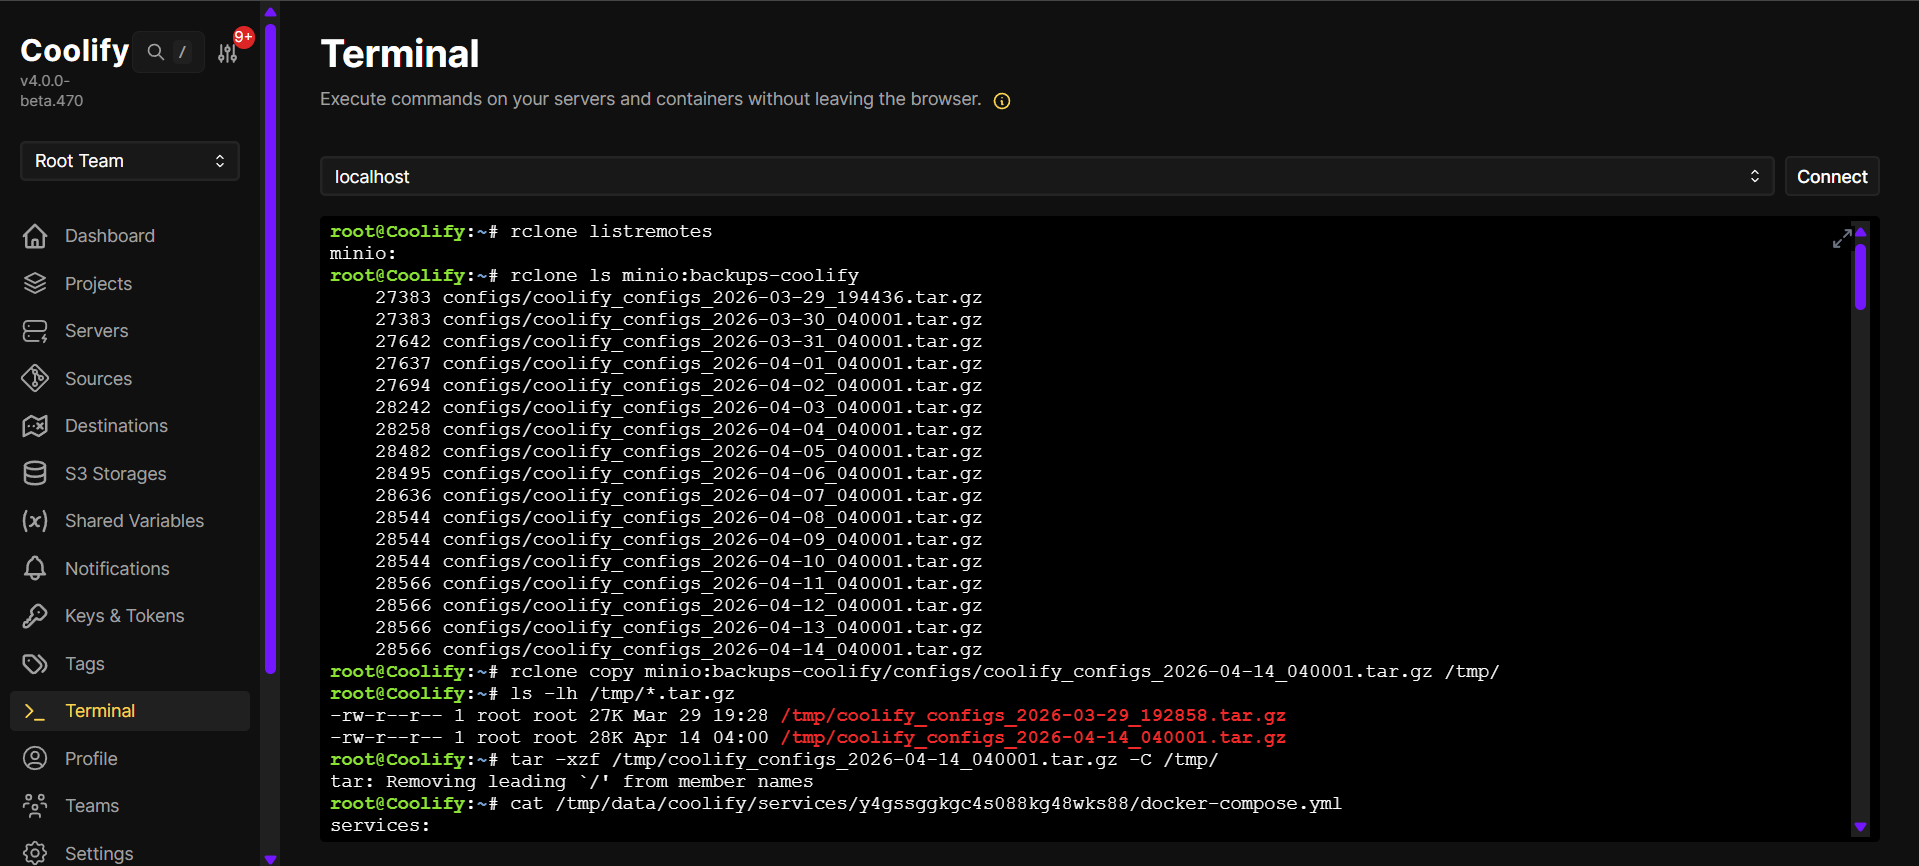
\includegraphics[width=\textwidth]{figuras/apendiceC/C2/apC_rclone.png}
    \caption[Ejecución de rclone en la terminal de Coolify]{Terminal integrada de Coolify mostrando el listado de respaldos disponibles en MinIO y la copia del archivo seleccionado al directorio temporal del servidor.}
    \label{fig:apC_rclone}
\end{figure}

\subsection{Identificación de servicios}

Coolify organiza los archivos de cada servicio bajo identificadores únicos. Las rutas críticas dentro del directorio extraído para el despliegue institucional son:

\begin{itemize}
    \item \textbf{Stack Documenso} (aplicación, base de datos y Browserless): \nolinkurl{/data/coolify/services/y4gssggkgc4s088kg48wks88/}
    \item \textbf{Servicio Socat}: \nolinkurl{/data/coolify/services/i040ggc0c84c0sc0ss4cs0co/}
\end{itemize}

Cada directorio contiene un archivo \texttt{docker-compose.yml} y un archivo \texttt{.env} con la definición de servicios y los secretos necesarios para su operación.

\subsection{Restauración desde la interfaz de Coolify}

Navegar en el panel de Coolify hacia \texttt{Proyecto Documenso} $\rightarrow$ \texttt{production} $\rightarrow$ \texttt{DocumensoProd} y seguir los pasos indicados a continuación.

\begin{enumerate}
    \item \textbf{Restaurar el archivo Compose.} Presionar el botón \textbf{Edit Compose File}. En el editor emergente (Figura~\ref{fig:apC_edit_compose}), reemplazar todo el contenido con el texto del archivo \texttt{docker-compose.yml} extraído en la ruta del identificador correspondiente y presionar \textbf{Save}.

    \begin{figure}[H]
        \centering
        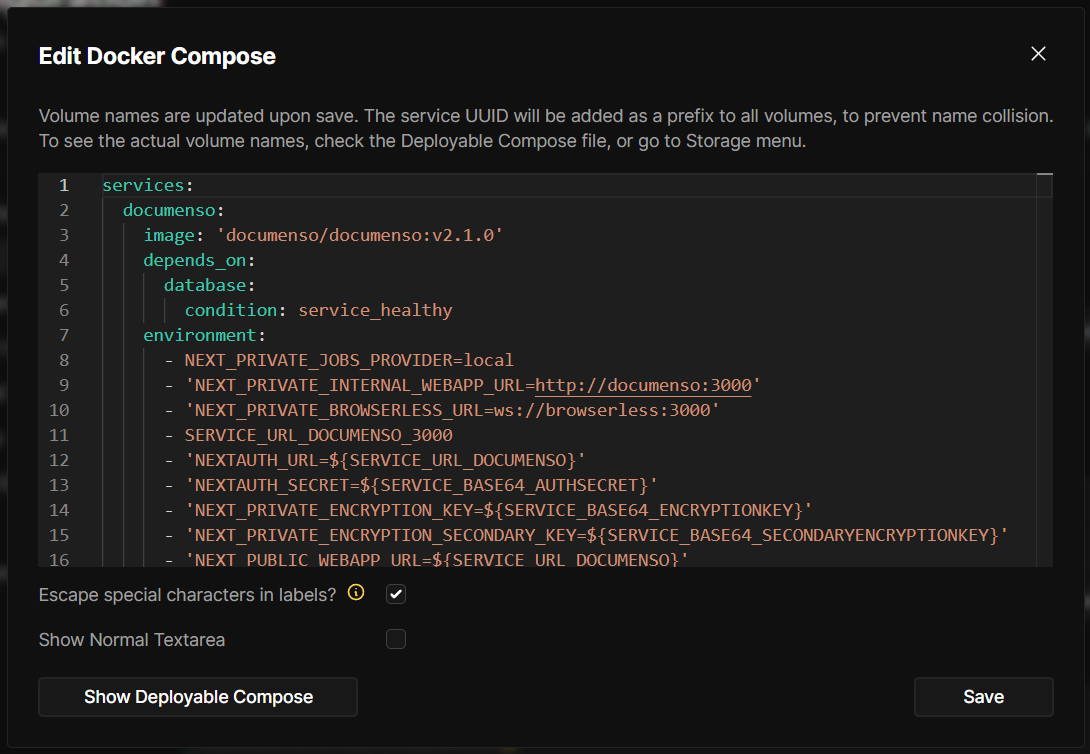
\includegraphics[width=\textwidth]{figuras/apendiceC/C2/apC-edit-compose.png}
        \caption[Editor de Docker Compose en Coolify]{Editor de la composición Docker accesible mediante \textbf{Edit Compose File} en Coolify, donde se reemplaza el contenido con la configuración recuperada del respaldo.}
        \label{fig:apC_edit_compose}
    \end{figure}

    \item \textbf{Restaurar las variables de entorno.} Ir a la pestaña \textbf{Environment Variables}, activar \textbf{Developer View} para obtener el editor de texto plano y pegar el contenido completo del archivo \texttt{.env} restaurado. Presionar \textbf{Save}.

    \item \textbf{Repetir para el servicio Socat.} Navegar al servicio del proxy Socat en Coolify y aplicar los pasos~1 y 2 con los archivos de su identificador (\texttt{i040ggc0c84c0sc0ss4cs0co}).

    \item \textbf{Desplegar y verificar.} Presionar \textbf{Deploy} en cada servicio. Tras el redespliegue, confirmar que los cuatro contenedores alcancen el estado \texttt{Healthy} en el panel de Coolify (Subsección~\ref{subsec:validacion_healthcheck}) y que el endpoint \nolinkurl{https://documentos.facet.unt.edu.ar/api/health} reporte \texttt{\char34 ok\char34} en todos sus campos.
\end{enumerate}

%----------------------------------------------------------------------------------------

\section{Renovación del Certificado de Firma Institucional}
\label{AppendixC:RenovacionCertificado}

Cuando el certificado autofirmado se aproxima a su fecha de caducidad, se debe generar un nuevo par de claves y reemplazar la variable de entorno correspondiente en Coolify. El certificado actual, generado durante el despliegue inicial, es válido hasta el 25 de marzo de 2036 (Apéndice~\ref{AppendixB:Crypto}).

\begin{enumerate}
    \item \textbf{Generar el nuevo material criptográfico.} Abrir una terminal en la computadora local del administrador y ejecutar los comandos de generación de clave privada, certificado X.509 y empaquetado PKCS\#12 detallados en la Sección~\ref{AppendixB:Crypto}. Al finalizar, se obtendrá un archivo de texto con la cadena codificada en Base64 del nuevo certificado. No es necesario ni recomendable ejecutar este procedimiento dentro del servidor de producción.

    \item \textbf{Actualizar la variable de entorno.} En la interfaz de Coolify, navegar a \texttt{Proyecto Documenso} $\rightarrow$ \texttt{production} $\rightarrow$ \texttt{DocumensoProd} y acceder a la pestaña \textbf{Environment Variables}. Ubicar la variable \texttt{CERTIFICADO\_P12\_BASE64} (Figura~\ref{fig:apC_env_cert}) y reemplazar su valor por la nueva cadena en Base64 generada en el paso anterior. Presionar \textbf{Update}.

    \begin{figure}[H]
        \centering
        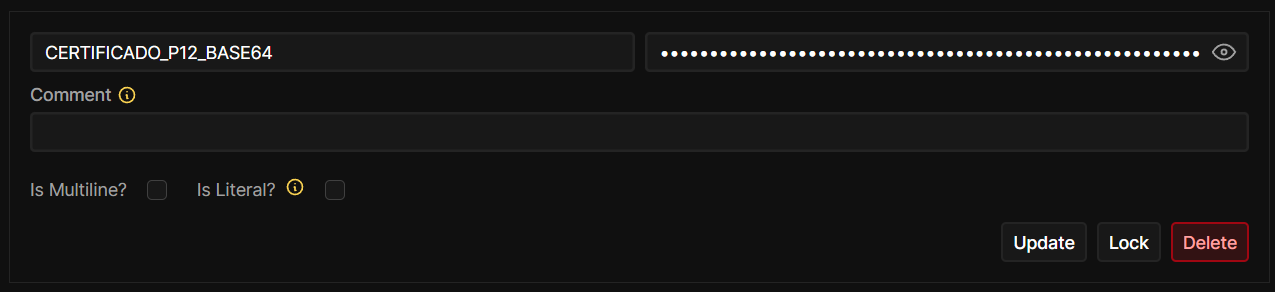
\includegraphics[width=\textwidth]{figuras/apendiceC/C3/apC-env-cert.png}
        \caption[Variable de entorno del certificado institucional en Coolify]{Variable \texttt{CERTIFICADO\_P12\_BASE64} en la pestaña \textbf{Environment Variables} de Coolify. El valor se muestra enmascarado por tratarse de un secreto.}
        \label{fig:apC_env_cert}
    \end{figure}

    \item \textbf{Actualizar la contraseña (condicional).} Si al generar el nuevo PKCS\#12 se utilizó una contraseña distinta a la original, también se debe actualizar el valor de la variable \texttt{SERVICE\_PASSWORD\_DOCUMENSO} en la misma pestaña.

    \item \textbf{Aplicar los cambios.} Presionar \textbf{Save} y luego \textbf{Deploy} para reiniciar el contenedor de Documenso con el nuevo certificado. El éxito de la operación se comprueba consultando el endpoint \nolinkurl{https://documentos.facet.unt.edu.ar/api/health} y verificando que el campo \texttt{certificate} reporte \texttt{\char34 ok\char34}.
\end{enumerate}

La renovación del certificado \textbf{no invalida ni corrompe} los documentos que ya fueron firmados con el certificado anterior. Cada PDF sellado conserva incrustada la firma y el certificado con el que fue emitido, por lo que su verificabilidad no depende del certificado activo en la plataforma. El nuevo certificado se utiliza exclusivamente para el sellado de los documentos que se procesen a partir del redespliegue.

%----------------------------------------------------------------------------------------

\section{Actualización de la Versión de Documenso}
\label{AppendixC:ActualizacionVersion}

Este procedimiento describe cómo actualizar Documenso a una versión más reciente dentro del entorno administrado por Coolify. Dado que la aplicación ejecuta migraciones de esquema de base de datos durante cada arranque, la operación exige un respaldo previo y la verificación de compatibilidad con el hardware del servidor.

\subsection{Prerrequisito crítico de hardware}

\textbf{Advertencia:} el servidor físico original de la FACET utiliza procesadores Intel Xeon E5620, que \textbf{no soportan instrucciones AVX}. Tal como se detalla en la Subsección~\ref{subsec:documenso_core}, a partir de la versión \texttt{v2.2.0} Documenso requiere AVX, por lo que el despliegue opera actualmente con \texttt{v2.1.0}, última versión compatible con este hardware.

\textbf{El procedimiento de actualización descrito en esta sección solo debe aplicarse si la infraestructura ha sido migrada a un servidor con CPU compatible con AVX.} Para verificar la compatibilidad del nuevo servidor, ejecutar el siguiente comando en la terminal del LXC:

\begin{lstlisting}[language=bash, caption={Verificación de soporte AVX en el procesador del servidor}, label={lst:apC_check_avx}]
lscpu | grep -i avx
\end{lstlisting}

Si el comando no devuelve ninguna línea con las \textit{flags} \texttt{avx} o \texttt{avx2}, el servidor \textbf{no es compatible} con versiones iguales o superiores a \texttt{v2.2.0}. La Figura~\ref{fig:apC_lscpu_avx} muestra el resultado de este comando en el hardware actual, donde la salida vacía confirma la ausencia de soporte AVX.

\textbf{Nota sobre virtualización:} si el nuevo servidor utiliza máquinas virtuales (por ejemplo, en Proxmox VE), el hipervisor puede ocultar las instrucciones AVX del procesador físico al usar perfiles de CPU genéricos como \texttt{kvm64}. Para evitar este problema, se debe configurar el modelo de CPU de la VM como \texttt{host}.

\begin{figure}[H]
    \centering
    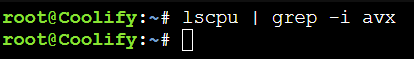
\includegraphics[width=0.5\textwidth]{figuras/apendiceC/C4/apC-lscpu-avx.png}
    \caption[Verificación de instrucciones AVX en el servidor actual]{Ejecución de \texttt{lscpu | grep -i avx} en el LXC del despliegue. La salida vacía confirma que el procesador Intel Xeon E5620 no soporta instrucciones AVX, lo que impide actualizar Documenso a versiones iguales o superiores a \texttt{v2.2.0}.}
    \label{fig:apC_lscpu_avx}
\end{figure}

\subsection{Preparación}

Antes de modificar cualquier archivo del despliegue, se deben completar dos tareas de preparación:

\begin{enumerate}
    \item \textbf{Consultar las notas de versión.} Revisar las \textit{Release Notes} oficiales en \url{https://github.com/documenso/documenso/releases} para la versión objetivo y todas las versiones intermedias entre la actual y la deseada. Identificar posibles \textit{breaking changes}, variables de entorno nuevas o eliminadas y requisitos adicionales de infraestructura.

    \item \textbf{Realizar un respaldo manual de la base de datos.} Documenso utiliza Prisma como ORM y ejecuta migraciones de esquema de forma automática durante el arranque de cada nueva versión. \textbf{Estas migraciones no son reversibles:} una vez aplicadas, el esquema de la base de datos queda adaptado a la versión nueva y no puede volver al estado anterior de forma automática. Por este motivo, es \textbf{estrictamente obligatorio} crear un respaldo manual de PostgreSQL desde Coolify antes de proceder. El procedimiento de respaldo y restauración se detalla en la Sección~\ref{AppendixC:RestauracionBD}.
\end{enumerate}

\subsection{Procedimiento de actualización en Coolify}

Una vez verificada la compatibilidad de hardware y completado el respaldo, la actualización se ejecuta desde la interfaz de Coolify:

\begin{enumerate}
    \item \textbf{Editar la composición Docker.} Navegar a \texttt{Proyecto Documenso} $\rightarrow$ \texttt{production} $\rightarrow$ \texttt{DocumensoProd} y presionar \textbf{Edit Compose File}. Localizar la línea de la imagen del servicio principal y modificar el \textit{tag} de versión:

    \begin{quote}
    \texttt{image: 'documenso/documenso:vX.Y.Z'}
    \end{quote}

    donde \texttt{vX.Y.Z} corresponde a la versión objetivo identificada en las notas de versión. Presionar \textbf{Save}.

    \item \textbf{Actualizar variables de entorno (condicional).} Si las notas de versión indican variables nuevas o modificadas, agregarlas o ajustarlas en la pestaña \textbf{Environment Variables} antes del despliegue.

    \item \textbf{Desplegar.} Presionar el botón \textbf{Deploy}. Coolify descargará la nueva imagen y recreará el contenedor. Durante el arranque, Prisma detectará las migraciones pendientes y las aplicará de forma automática sobre PostgreSQL. No se requiere intervención manual en la base de datos.
\end{enumerate}

\subsection{Verificación}

Tras el despliegue, el administrador debe confirmar que la actualización se completó correctamente:

\begin{enumerate}
    \item \textbf{Revisar los registros del servicio.} En Coolify, acceder a la pestaña \textbf{Logs} del servicio Documenso y verificar que las migraciones de Prisma hayan finalizado sin errores. Los mensajes indicativos de éxito incluyen líneas del tipo \texttt{All migrations have been successfully applied}.

    \item \textbf{Consultar el endpoint de salud.} Acceder a \nolinkurl{https://documentos.facet.unt.edu.ar/api/health} y verificar que los campos \texttt{status}, \texttt{database} y \texttt{certificate} reporten \texttt{\char34 ok\char34}.

    \item \textbf{Validación funcional.} Iniciar sesión en la interfaz web y comprobar que los documentos, firmantes y equipos existentes se muestren correctamente. Se recomienda ejecutar un ciclo de firma de prueba de extremo a extremo para confirmar la operación completa del sistema.
\end{enumerate}

\subsection{Procedimiento de rollback}

Si la actualización falla o produce un comportamiento inesperado, las migraciones de esquema aplicadas por Prisma \textbf{no se pueden revertir de forma automática}. Además, las políticas de reinicio automático de Docker provocan que el contenedor fallido intente arrancar de forma reiterada, y cada intento puede ejecutar migraciones parciales que corrompan la base de datos. Por este motivo, la primera acción debe ser detener el servicio antes de cualquier operación de restauración.

\begin{enumerate}
    \item \textbf{Detener el servicio fallido.} En el panel de Coolify, acceder a \texttt{DocumensoProd} y presionar el botón \textbf{Stop}. Esto detiene el contenedor de la aplicación y evita que siga intentando aplicar migraciones sobre la base de datos. \textbf{No detener el contenedor de PostgreSQL}, ya que debe permanecer activo para el paso siguiente.

    \item \textbf{Restaurar la base de datos.} Con el contenedor de la aplicación detenido, acceder al servicio \texttt{database} en Coolify y ejecutar el procedimiento de importación desde S3 descrito en la Sección~\ref{AppendixC:RestauracionBD}, utilizando el respaldo creado en la etapa de preparación.

    \item \textbf{Revertir la imagen.} Volver al servicio \texttt{DocumensoProd}, presionar \textbf{Edit Compose File} y restaurar el \textit{tag} de la imagen a la versión estable anterior (por ejemplo, \texttt{documenso/documenso:v2.1.0}). Presionar \textbf{Save}.

    \item \textbf{Redesplegar.} Presionar el botón \textbf{Deploy}. Coolify recreará el contenedor de la aplicación con la versión correcta y lo reconectará a la base de datos ya restaurada. Verificar la operación mediante el endpoint \texttt{/api/health} y una prueba funcional en la interfaz web.
\end{enumerate}

%----------------------------------------------------------------------------------------

\section{Diagnóstico de Fallas y Referencia Rápida}
\label{AppendixC:Diagnostico}

Esta sección reúne los puntos de inspección y las referencias necesarias para diagnosticar las fallas más frecuentes del despliegue.

\subsection{Monitoreo y registros}

El estado de salud y los registros de ejecución de los tres servicios del \textit{stack} ---Documenso, Browserless y PostgreSQL--- se consultan directamente desde la pestaña \textbf{Logs} de cada contenedor, accesible en Coolify mediante la ruta \texttt{Documenso} $\rightarrow$ \texttt{production} $\rightarrow$ \texttt{DocumensoProd}. Desde allí se pueden filtrar los mensajes por servicio para aislar el componente afectado.

\subsection{Tabla de resolución de problemas}

La Tabla~\ref{tab:apC_troubleshooting} resume los síntomas más comunes, el componente involucrado y la referencia al procedimiento o configuración correspondiente.

\begin{table}[H]
\centering
\caption[Referencia rápida de resolución de problemas]{Síntomas frecuentes del despliegue Documenso, componente a revisar y referencia al procedimiento o configuración correspondiente.}
\label{tab:apC_troubleshooting}
\small
\begin{tabular}{p{0.42\textwidth} p{0.52\textwidth}}
\hline
\textbf{Síntoma / Error} & \textbf{Componente a revisar / Referencia} \\
\hline
El endpoint \texttt{/api/health} reporta error en \texttt{database} & Estado del contenedor \texttt{database} en Coolify; verificar credenciales en el \texttt{.env}. \\[6pt]
El endpoint \texttt{/api/health} reporta error en \texttt{certificate} & El certificado caducó o el \texttt{BASE64} es inválido (Sección~\ref{AppendixC:RenovacionCertificado}). \\[6pt]
Los correos de invitación no llegan & Configuración SMTP y registros del contenedor Documenso (Sección~\ref{AppendixB:SMTP}). \\[6pt]
Error al procesar la firma o al cargar el editor de documentos & Registros del contenedor Browserless; verificar estado \texttt{Healthy} (Subsección~\ref{subsec:browserless}). \\[6pt]
\texttt{Illegal instruction (core dumped)} & Incompatibilidad de CPU con instrucciones AVX (Sección~\ref{AppendixC:ActualizacionVersion}). \\[6pt]
Documentos quedan en estado \texttt{PENDING} sin completarse & Registros del \textit{job} \texttt{internal.seal-document} (Subsección~\ref{subsec:browserless}). \\[6pt]
Carga de archivos falla con \texttt{413 Content Too Large} & Límite de \texttt{client\_max\_body\_size} en Nginx (Sección~\ref{sec:proxy_socat}). \\[6pt]
\texttt{Access Denied} al subir o descargar documentos & Credenciales S3 o política del \textit{bucket} en MinIO (Sección~\ref{AppendixB:S3}). \\[6pt]
Carga de archivos falla con error de almacenamiento o \texttt{Quota Exceeded} & Verificar y ampliar la cuota del \textit{bucket} desde la interfaz de MinIO (\texttt{Buckets} $\rightarrow$ \texttt{Quota}). \\
\hline
\end{tabular}
\end{table}

Para diagnósticos fuera de los escenarios listados, se puede consultar la guía oficial de resolución de problemas de Documenso en \url{https://docs.documenso.com/docs/self-hosting/maintenance/troubleshooting}.

%----------------------------------------------------------------------------------------

\section{Migración a Certificado Emitido por Autoridad Certificante (CA)}
\label{AppendixC:MigracionCA}

Tal como se establece en la Sección~\ref{sec:mecanismo_tecnico}, la arquitectura del sistema soporta de forma nativa certificados X.509 emitidos por Autoridades Certificantes licenciadas. Esta capacidad permite, sin modificar la infraestructura subyacente, migrar desde el esquema actual de firma electrónica con certificado autofirmado hacia un esquema de firma digital que cumpla el Artículo~9 de la Ley~25.506 \cite{ley25506}, si la institución lo requiriera en el futuro.

Las CA comerciales o gubernamentales suelen entregar el material criptográfico en archivos separados: clave privada, certificado del titular y cadena de confianza intermedia. Documenso requiere que estos componentes se empaqueten en un único contenedor PKCS\#12. El siguiente comando realiza esa operación:

\begin{lstlisting}[language=bash, caption={Empaquetado de certificado emitido por CA en formato PKCS\#12}, label={lst:apC_pkcs12_ca}]
openssl pkcs12 -export -out certificate.p12 \
    -inkey private.key \
    -in certificate.crt \
    -certfile chain.crt
\end{lstlisting}

Una vez obtenido el archivo \texttt{certificate.p12}, el procedimiento operativo es idéntico al de la Sección~\ref{AppendixC:RenovacionCertificado}: codificar el archivo en Base64, reemplazar el valor de la variable \texttt{CERTIFICADO\_P12\_BASE64} en Coolify y, si la frase de paso difiere de la actual, actualizar también \texttt{SERVICE\_PASSWORD\_DOCUMENSO}. Tras presionar \textbf{Deploy}, los documentos firmados a partir de ese momento llevarán un certificado reconocido por las cadenas de confianza de los lectores PDF estándar.

Para conversiones desde otros formatos de certificado (como DER o PEM sin cadena), se puede consultar la guía oficial de Documenso en \url{https://docs.documenso.com/docs/self-hosting/configuration/signing-certificate/local#using-an-existing-certificate}.
